% !TEX root = Thesis.tex

\chapter{Preliminaries}\label{chap:prelim}

  \newtheorem{defi}{Definition}

  In this section, we first raise the motivation to utilize triangulation for analog layout migration in Chapter~\ref{sec:WhyCDT}, and later review the planar straight-line graph (PSLG) and the corresponding constrained Delaunay triangulation (CDT)~\cite{CDT} in Chapter~\ref{sec:Review}. In the end, we define the analog layout prototyping problem in Chapter~\ref{sec:problem}.

  \section{Routing Preservation with Planar Triangulation}\label{sec:WhyCDT}

    To facilitate the routing preservation in the existing layout, the relationship between routing wires and placement blocks is crucial. The triangulation of layout plane is used to take down the correlation. Fig.~\ref{fig:WhyCDT} depicts that the updated triangular edges can retain the routing behavior among blocks after shrinking and stretching. Therefore, planar triangulation is applied to our analog layout migration mechanism.

    \begin{figure}[ht]
      \begin{center}
        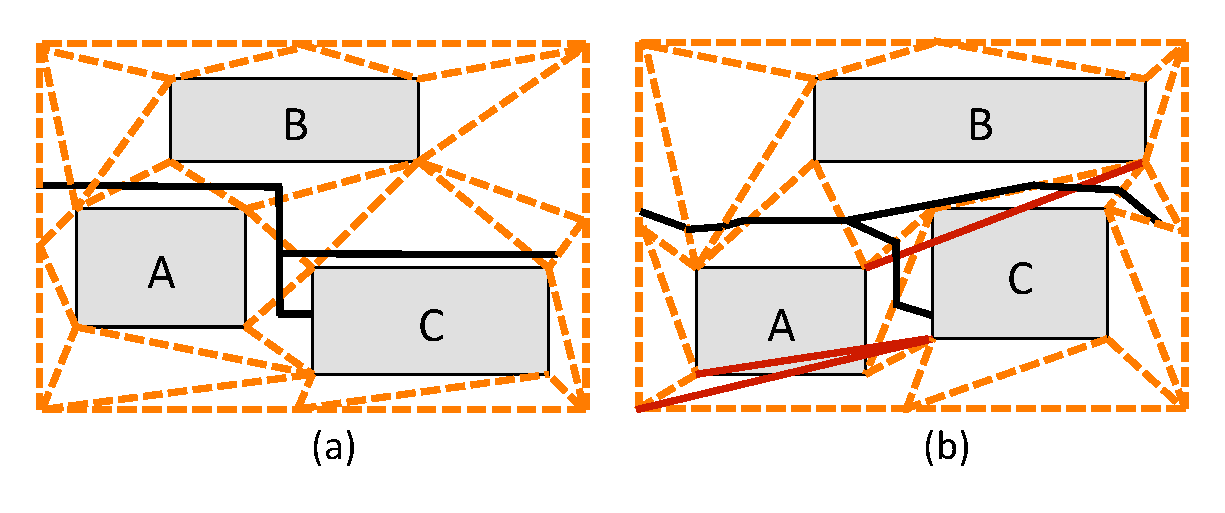
\includegraphics[width=\textwidth]{Fig/WhyCDT.eps}
        \caption{Illustration of triangulation to take down the correlation between placement and routing. (a). The existing layout with triangles at routing channel. (b) The migrated layout with updated triangular edges and recovering routing paths.}
        \label{fig:WhyCDT}
      \end{center}
    \end{figure}